\documentclass{beamer}
\usetheme{Warsaw}
% \usepackage{beamerthemesplit} // Activate for custom appearance

\addtobeamertemplate{navigation symbols}{}{%
    \usebeamerfont{footline}%
    \usebeamercolor[fg]{footline}%
    \hspace{1em}%
    \insertframenumber/\inserttotalframenumber
}

%\setbeamertemplate{navigationsymbols}{}
\usenavigationsymbolstemplate{}
\usepackage{amsmath, amssymb, setspace, amsthm, stackrel}
\usepackage{arydshln}

% graphics stuff
\usepackage{graphicx}
\usepackage{caption}
\usepackage{subcaption}
\captionsetup{compatibility=false}
%\usepackage{tabularx}

% Bibtex related stuff
\usepackage{natbib}
\bibpunct{(}{)}{;}{a}{}{,}


\newtheorem{thm}{Theorem}
\newtheorem{remarks}{Remarks}
%%%%%%%%%%%%%%%%%%%%%%%%%%%%%%%%%%%%%%%%%%%%%
% list of user-defined commands
%%%%%%%%%%%%%%%%%%%%%%%%%%%%%%%%%%%%%%%%%%%%
\renewcommand{\L}{\mathcal{L}}
\renewcommand{\S}{\mathcal{S}}
\renewcommand{\P}{\mathcal{P}}
\newcommand{\A}{\mathcal{A}}
\newcommand{\C}{\mathcal{C}}
\newcommand{\X}{\mathcal{X}}
\newcommand{\Y}{\mathcal{Y}}
\newcommand{\T}{\mathcal{T}}
\newcommand{\N}{\mathcal{N}}
\newcommand{\Tmat}{\mathbf{T}}
\newcommand{\Rmat}{\mathbf{R}}
%\renewcommand{\H}{\ensuremath{\mathcal{H}}}
\newcommand{\R}[1]{\ensuremath{ R_{#1} }}
%\newcommand{\RR}[2]{\ensuremath{ R_{#1<#2>} }}
\renewcommand{\H}{\mathcal{H}}
%\newcommand{\HH}[2]{\ensuremath{ R_{#1<#2>} }}
\newcommand{\tsum}{\ensuremath{\oplus}}
\newcommand{\tprod}{\ensuremath{\otimes}}
\newcommand{\tminus}{\ensuremath{\ominus}}
\newcommand{\Real}{\ensuremath{ \mathbb{R} }}
\newcommand{\norm}[1]{\left\|#1\right\|}
\newcommand{\bbeta}{\boldsymbol\beta}
\newcommand{\balpha}{\boldsymbol\alpha}
\newcommand{\bgamma}{\boldsymbol\gamma}
\newcommand{\bepsilon}{\boldsymbol\epsilon}
\newcommand{\blambda}{\boldsymbol\lambda}
\newcommand{\wh}[1]{\widehat{#1}}
\newcommand{\inner}[2]{\langle #1, #2 \rangle}

\newcommand{\hk}{H(R)}
\newcommand{\hkk}{H(R\otimes R)}



\title{Functional Data Analysis Approach to Land Cover Classification in India Using MERIS Terrestrial Chlorophyll Index Data}
		
\author[]{Daniel Fortin \\[0.5cm]
Iowa State University}	
		
\date{November 18, 2014}

\begin{document}

\frame{\titlepage}

%%%%%%%%%%%%%%%%%%%%%%%%%%%%%%%%%%%%%%%%%%%
%%% INTRODUCTION 
%%%%%%%%%%%%%%%%%%%%%%%%%%%%%%%%%%%%%%%%%%%

\begin{frame}[t]{Functional Data Analysis (FDA)}
	All data are discrete, so why adopt an FDA approach to analysis?

	\begin{quote}
 A functional data analysis approach is attractive when a primary variable of interest is best conceptualized as realizations of random smooth curves whose features require flexible estimation.
	\end{quote}
	FDA is often used when:
	\begin{itemize}
		\item Observations are at such a high frequency that it makes practical sense to treat it as a continuos variable
		\item Scientific questions of interest relate to properties of curves (e.g. derivatives)
		\item Estimation or prediction of the whole process is desired over a scalar summary of the curve
	\end{itemize}
\end{frame}
%--- Next Frame ---%
% \begin{frame}[t]{Example: Human Growth Curves}
% 	\begin{figure}
% 	\begin{center}
% 	\includegraphics[width=0.8\textwidth]{Plots/growth-curves.png}
% 	\caption{ The heights of 10 girls measured at 31 ages.}
% 	\end{center}
% 	\end{figure}
% \end{frame}
%--- Next Frame ---%

% \begin{frame}[t]{Example: Temperature Profiles at Canadian Weather Stations}
% 	\begin{figure}
% 	\begin{center}
% 	\includegraphics[width=3in]{Plots/canadian-weather.pdf}
% 	\caption{ Mean monthly temperatures for Canadian weather stations.}
% 	\end{center}
% 	\end{figure}
% \end{frame}

%--- Next Frame ---%

% \begin{frame}[t]{Example: Oceanography measurements}
% 	\begin{figure}
% 	\begin{center}
% 	\includegraphics[width=\textwidth]{Plots/Nerini-figure.png}
% 	\caption{Example of temperature profiles sampled by elephant seal and spatial location of sampled curves along trajectory (white circles).The cruise duration is 1 month. During the travel, the animal crosses and samples heterogeneous water structures. (Nerini 2010)}
% 	\end{center}
% 	\end{figure}
% \end{frame}
%--- Next Frame ---%

% \begin{frame}[t]{}
% 	\begin{tabular}{c|c|c|}
% 		& Independent & Dependent \\
% 		\hline
% 		Sparse & \includegraphics[width=1.3in]{Plots/Nerini-figure-2.png} & \includegraphics[width=1.3in]{Plots/Nerini-figure-2.png} \\
% 		\hline
% 		Dense & \includegraphics[width=1.3in]{Plots/growth-curves.png} &\includegraphics[width=1.3in]{Plots/canadian-weather.pdf}\\
% 		\hline
% 	\end{tabular}
% \end{frame}

% \frame{
% \begin{figure}
%         \centering
%         \begin{subfigure}[b]{0.44\textwidth}
%                 \centering
%                 \includegraphics[width=\textwidth]{Plots/fourier-basis-7.pdf}
%                 \caption{Fourier basis functions}
%         \end{subfigure}
%          \begin{subfigure}[b]{0.44\textwidth}
%                 \centering
%                 \includegraphics[width=\textwidth]{Plots/bspline-basis-7-order4.pdf}
%                 \caption{B-spline basis functions}
%         \end{subfigure}
%  \end{figure}
% }
%--- Next Frame ---%

%%%%%%%%%%%%%%%%%%%%%%%%%%%%%%%%%%%%%%%%%%%%%%%%%%%
%%% Phenology Data: Description and analysis goals
%%%%%%%%%%%%%%%%%%%%%%%%%%%%%%%%%%%%%%%%%%%%%%%%%%%

\begin{frame}
\frametitle{Studying Annual Life-cycles of Vegetation with MERIS Terrestrial Chlorophyll Index (MTCI)}
\begin{itemize}
\item \emph{Phenology} is the study of annual life-cycles of terrestrial vegetation and how they are affected by climate change or other environmental variables.

\item Understanding vegetation phenology and its spatio-temporal variation is required to reveal and predict ongoing changes in Earth system dynamics. \\[0.5cm]

\item MTCI Data: Observations of chlorophyll content via satellite
\begin{itemize}
	\item Temporal resolution = 8 days
	\item Spatial resolution = 4.6 km by 4.6 km
	\item Area is a subregion of India
	\item Time period 2003 - 2007
\end{itemize}
\end{itemize}
\end{frame}

\begin{frame}[t]{Study region in southern India: (Image from May 2000)}
	\includegraphics[width=0.95\linewidth]{Images-phenology-fda/Satellite/India_zoom.png}
\end{frame}
%--- Next Frame ---%

\begin{frame}[t]{GLC2000 Global Land Cover classification \\@ 4.6 km by 4.6 km spatial resolution}
	\begin{figure}
		%\includegraphics[width=0.35\linewidth]{Images-phenology-fda/Satellite/India-5-12-2000.png}
		\includegraphics[width=\linewidth]{Images-phenology-fda/land_cover.pdf}
		%\caption{Land cover classification at 4.6~km spatial resolution derived from GLC2000 land cover database.} \label{fig:land cover}
	\end{figure}
\end{frame}
%--- Next Frame ---%

\frame
{
\frametitle{Defining Annual Vegetation Life-cycles}
\begin{figure}
   \begin{center}
   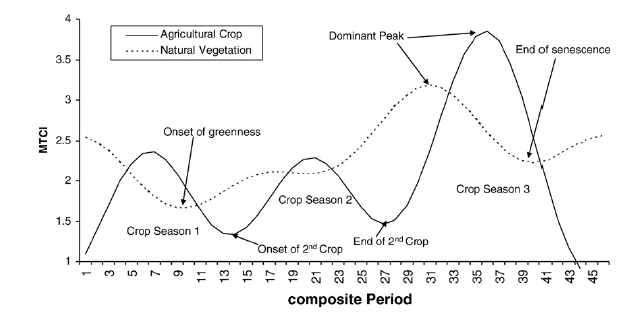
\includegraphics[width=\linewidth]{Plots/PhenoVars_Jegan.png}
   %\caption{Diagram illustrating typical phenology patterns for agricultural land and natural vegetation. }
\end{center}
\end{figure}
}

\begin{frame}[t]{Mean MTCI by landcover for 2003 - 2007}
	\begin{figure}
		\includegraphics[width=\linewidth]{Images-phenology-fda/mean_by_LC_facet_year.pdf}
		%\caption{Land cover classification at 4.6~km spatial resolution derived from GLC2000 land cover database.}
	\end{figure}
\end{frame}
%--- Next Frame ---%

\frame
{
\frametitle{Data processing and analysis flow chart }
\begin{figure} %  figure placement: here, top, bottom, or page
   \begin{center}
   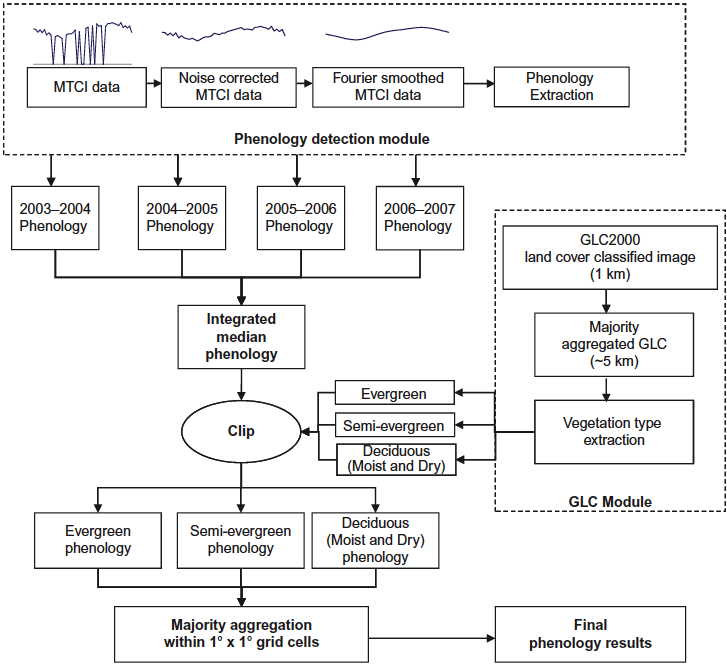
\includegraphics[width=0.7\linewidth]{Plots/PhenoScheme.png}
%   \caption{example caption}
   %\label{fig:example}
   \end{center}
\end{figure}
}


\begin{frame}[t]{Global Land Cover 2000 (GLC2000) project}
\begin{itemize}
	\item GLC2000 is a global landcover map created in 2000 in a massive collaborative effort.
	\item 26 landcover categories
	\item 1 km by 1 km spatial resolution
	\item We have data on proportion of each landcover category in each of the MTCI spatial grid cells
	\item Landcover for MTCI data is derived from GLC2000 map by assigning landcover with largest proportion
\end{itemize}
		\begin{figure}
		\includegraphics[width = 0.5\textwidth]{Images-phenology-fda/Plots/proportion_agriculture.pdf}
		\caption{Proportion of agricultural landcover using GLC2000 database}
		\end{figure}

\end{frame}
%--- Next Frame ---%


\begin{frame}[t]{Modeling Approach}
	 Our approach consists of the following steps:
	\begin{enumerate}
		\item Label each cell as either \textbf{Vegetation}, \textbf{Agriculture}, or \textbf{other}.
		\item Derive an empirical basis by estimating functional principal components from locations that primarily agricultural landcover.
		\item Project annual MTCI data at each location onto this basis, reducing the information for each curve to a low dimensional vector of coefficients.
		\item Classification is performed using multivariate techniques by viewing basis coefficients as multivariate random variable.
		\begin{itemize}
			\item Use homogeneous agriculture cells and homogeneous vegetation cells as training set.
		\end{itemize}
	\end{enumerate}
\end{frame}

\begin{frame}[t]{Agriculture and Natural Vegetation Land Cover}
	\begin{minipage}{0.48\textwidth}
		\begin{figure}
		\includegraphics[width = \textwidth]{Images-phenology-fda/Plots/proportion_agriculture.pdf}
	%	\caption{Proportion of agricultural landcover using GLC2000 database}
		\end{figure}
	\end{minipage}
	\begin{minipage}{0.48\textwidth}
		\begin{figure}
		\includegraphics[width = \textwidth]{Images-phenology-fda/Plots/landcover_ag_veg.pdf}
	%		\caption{Black pionts are homogeneous agriculture locations}
		\end{figure}
	\end{minipage}

	\begin{minipage}{0.48\textwidth}
	\begin{itemize}
		\item Proportion Agriculture
		\item based on GLC2000 database
	\end{itemize}
	\end{minipage}
	\begin{minipage}{0.48\textwidth}
	\begin{itemize}
		\item black points indicate homogeneous agriculture cells
		\item homogeneous agriculture = 100\% agriculture landcover
	\end{itemize}
	\end{minipage}
\end{frame}
%--- Next Frame ---%


%%%%%%%%%%%%%%%%%%%%%%%%%%%%%%%%%%%%%%%%%%%%%%%%%%%%
%%% Covariance function and FPC estimation
%%%%%%%%%%%%%%%%%%%%%%%%%%%%%%%%%%%%%%%%%%%%%%%%%%%
\begin{frame}[t]{Methodology}
	\textbf{Process Model:}
	 Trajectories $X_s(t)$, $t \in [a,b]$ are second order stochastic process with mean $\mu(t)$ and bivariate temporal covariance function
	\begin{equation*}
		C_{0}(t',t)=E([X(t')-\mu(t')][X(t)-\mu(t)])
	\end{equation*}
	\begin{itemize}
		\item $t',t\in [a,b]$
		\item $X_s(t)$ are smooth in that they take values in a reproducing kernel Hilbert space (RKHS) $\H$
		\item inner product $\inner{f}{g}_{\H}$ and r.k. $R(t',t)$
		\item $\H= \{f : f, f' \mbox{ absolutely continuous}, f'' \in L_2([a,b])\}$
	\end{itemize}

\end{frame}
%--- Next Frame ---%

\begin{frame}[t]{Methodology}
	\textbf{Observation Model:}
	Let $X_{s_1}(t), \dots, X_{s_N}(t)$ collection of realizations of $X_s(t)$.
	We model observed values $Y_s(t_{ij})$ as
	\begin{equation*}
		Y_{s_i}(t_{ij})=X_s(t_{ij})+\epsilon_{ij},\mbox{ }j=1,\dots,m;\mbox{ }i=1,\dots,N,
	\end{equation*}
	\begin{itemize}
		\item $s_i$ indexes spatial location
		\item $j$ indexes discrete observations on a curve
		\item $t_{ij} \sim \mbox{ iid on }[a,b]$
		\item `time' observations can be different across curves
		\item $\epsilon_{ij}$ are iid errors with mean zero and variance $\sigma_{0}^{2}.$
		\item $X_s(t)$ and $\epsilon_{ij}$ are mutually independent.
	\end{itemize}
\end{frame}
%--- Next Frame ---%

% \begin{frame}[t]{Some Background on Reproducing Kernel Hilbert Space}
% 	Spaces generated by positive definite functions
% 	\begin{itemize}
% 	\item Let $K(x,y)$ be a symmetric positive-definite kernel function.
% 	\item $\H_K = \{K(\cdot, y), y \in \Real\}$
% 	\end{itemize}
% 	From Mercer's theorem $K(x,y)$ has the representation
% 	\[K(x,y)=\sum_{i=0}^{\infty}\lambda_{i}\phi_{i}(x)\phi_{i}(y)\]
% 	\begin{itemize}
% 	\item $\phi_{i}$ are eigenfunctions of the kernel function $K$
% 	corresponding to eigenvalues $\lambda_{i}$.
% 	\item $\phi_{i}$ are basis for $L_2$.
% 	\end{itemize}
% 	$\H_{K}\subset L_{2}$ contains functions satisfying
% 	\[f(x)=\sum_{i=1}^{\infty}c_{i}\phi_{i}(x)\]
% 	 for $c_{i} \mbox{ with  }\norm{f}_{\H_K}:= 	\sum_{i=1}^{\infty}\frac{{c_{i}^{2}}}{\lambda_{i}}<\infty$
% \end{frame}
%--- Next Frame ---%

\begin{frame}{Some Background on Reproducing Kernel Hilbert Space}
The reproducing property:
\begin{itemize}
\item $f(x_i) = \inner{K(\cdot, x_i)}{f}$
\item $\inner{K(\cdot, x_i)}{K(\cdot, x_j)} = K(x_i, x_j)$
\end{itemize}
implies that for $f(x)=\sum_{i=1}^{N}b_{i}K(x,x_{i})$
\[\left\Vert f\right\Vert _{H_{K}}^{2}=\inner{f}{f}_{H_{K}}=\sum_{i=1}^{N}\sum_{j=1}^{N}b_{i}b_{j}K(x_{i},x_{j})\]
\end{frame}
%--- Next Frame ---%

\begin{frame}\frametitle{Cai and Yuan (2010)}
	\begin{thm}
Assume the sample path of $X$ belongs to an RKHS $H_{R}.$ Then the covariance function $C_{0}(s,t)$ belongs to the tensor product space $H(R\otimes R)=H(R)\otimes H(R)$,
an RKHS associated with reproducing kernel
\[
R\otimes R((s_{1},t_{1}),(s_{2},t_{2}))=R(s_{1},s_{2})R(t_{1},t_{2}).
\]
\end{thm}
This result motivated the following estimator
\begin{equation*}
\hat{C}_{\lambda}=\stackrel[C \in \H\otimes\H]{}{\mbox{argmin}} \{l_{n}(C)+\lambda\left\Vert C\right\Vert _{\H\otimes \H}^{2}\},
\end{equation*}
 where
\begin{equation*}
l_{n}(C)=\sum_{i=1}^{n}\sum_{1\leq j_{1}\neq j_{2}\leq m}([Y_{ij_{1}}-\mu_{0}(t_{ij_1})][Y_{ij_{2}}-\mu_{0}(t_{ij_{2}})]-C(t_{ij_{1}},t_{ij_{2}}))^{2}
\end{equation*}
\end{frame}

\begin{frame}[t]{Covariance estimator}
	\textbf{Remarks:}
	\begin{itemize}
		\item $\hat{C} \rightarrow C_0$ at the rate
		\[
			O_p\left(\left(\frac{log n}{nm}\right)^{2\alpha/(2\alpha + 1)} + \frac{1}{n}\right)
		\]
		under integrated squared error when $X(t)$ is $\alpha$ times differentiable ($\alpha > 1/2$).
		\item Allows explicit calculation of FPCs
		\item Smoothing parameter selection is performed using 5-fold cross validation
	\end{itemize}
\end{frame}
%--- Next Frame ---%

\begin{frame}[t]{Spatially re-weighted covariance function estimator}

	\textbf{Basic principle of spatial statistics}: data in closer proximity have stronger correlation and contribute similar information.

	\textbf{Idea:} down weight data which are more correlated and provide redundant information

	\textbf{approach:}
	\begin{itemize}
		\item Denoted the point intensity at location $k$ by $\gamma_k$
		\item define a weight function
	\begin{equation*}
		w_k = \left(\frac{1}{\gamma_k}\right)^p,
	\end{equation*}
	where $p$ is a scale parameter connected to the strength of dependence.
	\end{itemize}


\end{frame}
%--- Next Frame ---%

\begin{frame}[t]{Spatially re-weighted covariance estimator}
	\begin{equation*}
	\hat{C}_{\lambda}=\stackrel[C \in \H\otimes\H]{}{\mbox{argmin}} \{l_{n}(C)+\lambda\left\Vert C\right\Vert _{\H\otimes \H}^{2}\},
	\end{equation*}
	 where
	\begin{equation*}
	l_{n}(C)=\sum_{i=1}^{n}\sum_{1\leq j_{1}\neq j_{2}\leq m}w_i([Y_{ij_{1}}-\mu_{0}(t_{ij_1})][Y_{ij_{2}}-\mu_{0}(t_{ij_{2}})]-C(t_{ij_{1}},t_{ij_{2}}))^{2}
	\end{equation*}
	\begin{itemize}
	\item for independent data, $p = 0 \rightarrow$ $w_i = 1$ for all locations.
	\item Simulations (on next slide) indicate $p$ near $1/2$ works well.
	\end{itemize}
\end{frame}

%--- Next Frame ---%

\begin{frame}[t]{Simulations}
	We generate functional data as
	\begin{equation*}
		X_s(t) = \sum^{3}_{k=1}\zeta_k Z_k(s) \cos(k\pi t) \hspace{0.5cm} t \in [0,1],
		\label{eq:sim process2}
	\end{equation*}
	where \(\zeta_k=(-1)^{k+1}k^{-2}\). The random variables $Z_k(s)$ are sampled from a Gaussian random field with $E[Z_k(s)]=0$ and
	\begin{equation*}
		Cov(Z_k(s_i), Z_j(s_l)) = \begin{cases}
																	e^{-\norm{s_i - s_l}/r} &\mbox{ if } k = j\\
																	0 & \mbox{ if } j \neq k.
																\end{cases}
	\end{equation*}

	\begin{equation*}
		Y^{(k)}_{ij}(t_{ij}) = X_{ij}(t_{ij}) + \epsilon_{ij}, \mbox{ } i = 1, \dots, 68; j = 1, \dots, 20; k = 1, \dots, 100,
	\end{equation*}
	where $\epsilon_{ij} \sim N(0, 0.01^2)$


\end{frame}
%--- Next Frame ---%

\begin{frame}[t]{Simulation Results}

		varying the range parameter $r \in \{0.1, 0.2, 0.3\}$ and the weight parameter $p \in \{0, 1/3, 1/2, 1\}$.

		\begin{equation*}
			L = \frac{1}{100}\sum_{k=1}^{100}\int_{[0,1]^2} [\hat{C}^{(k)}(t_1, t_2) - C(t_1,t_2)]^2dt_1dt_2.
		\end{equation*}
	\begin{minipage}{0.48\textwidth}
		\begin{figure}[h]
			\begin{center}
				\includegraphics[width=\textwidth]{Images-ordinary-kriging/Plots/grid.pdf}
			\end{center}
			%\caption{Locations of curves used for the simulation.} \label{fig:grid3}
		\end{figure}
	\end{minipage}
\begin{minipage}{0.48\textwidth}
		% plots of MSE vs spatial weight values for different values of spatial dependence
		\begin{figure}[h]
			\begin{center}
				\includegraphics[width=1.3\textwidth]{Images-ordinary-kriging/Plots/MSE_trends.pdf}
			\end{center}
		\end{figure}
	\end{minipage}

\end{frame}
%--- Next Frame ---%

\begin{frame}
	\frametitle{Functional Principal Components}
	To the covariance $C(s,t)$ has the following representation
	\begin{equation*}
	 C(s,t) = \sum_{i=1}^{\infty}\lambda_i\psi_i(s)\psi_i(t),
	\end{equation*}
	\begin{itemize}
	\item  $\{\psi_m(t)\}_{m=1,2,\ldots}$ are orthonormal (in $L_2$) eigenfunctions
	\item  $\{\lambda_m \}_{m=1,2,\ldots}$ are nonnegative and nondecreasing eigenvalues.
	\item eigenfunctions satisfy $\int_a^bC(s,t)\psi_j(t)dt = \lambda_j\psi_j(t)$.
	\end{itemize}
	Karhunen-Loeve theorem $\rightarrow$ $X(t)$ admits the representation
	\begin{equation*}
	X(t) =  \sum_{m=1}^{\infty}\alpha_m \psi_m(t), \mbox{ where  } \alpha_m = \int_a^b X(t) \psi_m(t)dt,
	\end{equation*}
	\begin{itemize}
	\item $\{\alpha_m \}_{m=1,2,\ldots}$ are uncorrelated random variables
	\item $E(\alpha_m)=0$ and Var($\alpha_m$) = $\lambda_m$, $\sum_m \lambda_m < \infty$.
	\end{itemize}
\end{frame}

\frame{
\frametitle{Functional Principal Components Estimate}
We seek functions $\hat{\psi}(s)$ that satisfy
\begin{equation*} \label{eq:eigenfuns}
\int \hat{C}(s,t)\hat{\psi}(t)dt=\theta\hat{\psi}(s).
\end{equation*}
\begin{itemize}
\item Let $\mathbf{g(\cdot)}=(1, k_1(\cdot),R_{1}(\cdot, t_1),R_{1}(\cdot, t_2),\dots, R_{1}(\cdot, t_K))'.$
\item We show that $\hat{C}(s,t)= \mathbf{g}(s)'A\mathbf{g}(t)$ for a known matrix $A$.
\end{itemize}
The following result states that the eigenfunctions can be expressed as a linear combination of the elements of $\mathbf{g}$.
}


\frame{
\frametitle{Functional Principal Components Estimate}
\begin{thm}
	The eigenfunctions of $\hat{C}(s,t)$ can be expressed as
	\begin{equation*}
		\hat{\psi}_k(\cdot) = b'_k\mathbf{g}(\cdot),
	\end{equation*}
	where $Q$ is defined to be
\begin{equation*}
	Q_{ij} = \int_0^1\mathbf{g_i}(t)\mathbf{g}_j(t)dt,
\end{equation*}
	$b_k$ is the $k$-th column of $B=Q^{-1/2}U$ and $U$ is the eigenvectors of $Q^{1/2}AQ^{1/2}$, and
\[
\mathbf{g(\cdot)}=(1, k_1(\cdot),R_{1}(\cdot, t_1),R_{1}(\cdot, t_2),\dots, R_{1}(\cdot, t_K))'.
\]
\end{thm}
}

% \frame{
% \frametitle{Covariance function and FPC estimation}
% \textbf{Remarks: }
% \begin{itemize}
% \item  Allows smoothing penalty to be more directly connected to the curves (i.e. the scientific process being observed).
% \item Simulations indicate the estimator performs well even with sparsely observed curves.
% \item Method is general and could easily be applied to a penalty based on arbitrary linear differential operators.
% \item We have also created an R package implementation, making it convenient to use empirical basis representation for functional data analyses.
% \end{itemize}
% }

%--- Next Frame ---%

%%%%%%%%%%%%%%%%%%%%%%%%%%%%%%%%%%%%%%
%%% Classification Model
%%%%%%%%%%%%%%%%%%%%%%%%%%%%%%%%%%%%%%

\begin{frame}[t]{Representing curves in FPC basis}
	To produce smooth representation of the trajectories $X_i(t)$, project the observations $Y_i(t_j), j = 1, \dots, 46$ onto the finite dimensional functional basis
	\[
	\{\hat{\psi}_k(t), k = 1, \dots, q\},
	\]
where $q$ is chosen such that at least $90\%$ of the variation is explained.
	\begin{equation*}
		\widehat{X_i(t)} = \sum_{k=1}^q\alpha_{k,i} \hat{\psi}_k(t) = \boldsymbol{\alpha_i'}\boldsymbol{\psi}.
		\label{phen:coef}
	\end{equation*}
	\begin{itemize}
		\item $\balpha$ is a coefficient vector that depends on location
		\item $\psi_k(t)$ does not depend on location
	\end{itemize}

\end{frame}
%--- Next Frame ---%

\begin{frame}[t]{Classification Model}
	\textbf{Linear Discriminant Analysis (LDA)} % (fold)

	Let C be a random variable taking values in $\mathcal{C} = \{ \text{Agriculture}, \text{Vegetation}\} = \{\text{A}, \text{V}\}$.
	\begin{equation*}
		\hat{\text{C}}(\boldsymbol{\alpha}) =
		\begin{cases}
				\text{A} \hfill & \text{ if } \text{Pr}(\text{C = A }| \boldsymbol{\alpha})> \text{Pr}(\text{C = V }| \boldsymbol{\alpha})\\
				\text{V} \hfill & \text{ otherwise}
		\end{cases}
	\end{equation*}
	Computation of the posterior probabilities follows from modeling the class-conditional densities $f_k(\boldsymbol\alpha)$ as multivariate Gaussian distributions
	\begin{equation*}
		f_k(\boldsymbol\alpha) = \frac{1}{(2\pi)^{p/2}}e^{-\frac{1}{2}(\boldsymbol\alpha - \boldsymbol\mu_k)^T\Sigma^{-1}(\boldsymbol\alpha - \boldsymbol\mu_k)}
	\end{equation*}
	LDA assumes common covariance matrix between classes.
	\begin{equation*}
		\text{Pr}(\text{C} = \text{A } | \boldsymbol\alpha) = \frac{f_{A}(\boldsymbol\alpha)\pi_{A}}{f_{A}(\boldsymbol\alpha)\pi_{A}+f_{V}(\boldsymbol\alpha)\pi_{V}}
	\end{equation*}
	where $\pi_{A}$ and $\pi_{V}$ are the prior probabilities class membership.
\end{frame}
%--- Next Frame ---%

%%%%%%%%%%%%%%%%%%%%%%%%%%%%%%%%%%%%%
%%% RESULTS AND CONCLUSIONS
%%%%%%%%%%%%%%%%%%%%%%%%%%%%%%%%%%%%%

\begin{frame}[t]{FPC Estimation: 2003 - 2007}
	\begin{minipage}{0.5\textwidth}
	\begin{figure}
	\includegraphics[width =\textwidth]{Images-phenology-fda/PCF_all_years.pdf}
	\end{figure}
	\end{minipage}
	\begin{minipage}{0.46\textwidth}
		\begin{itemize}
			\item First three FPCs estimated separately for each year
			\item Number of FPCs chosen to capture at least 90\% of variation
		\end{itemize}
	\end{minipage}
\end{frame}
%--- Next Frame ---%

\begin{frame}{Classification Results}
	\begin{minipage}{0.45\textwidth}
		\begin{figure}
		\includegraphics[width = \textwidth]{Images-phenology-fda/Plots/prob_ag.pdf}
		\caption{Posterior probability of `Agriculture'}
		\end{figure}
	\end{minipage}
	\begin{minipage}{0.45\textwidth}
		\begin{figure}
		\includegraphics[width = \textwidth]{Images-phenology-fda/Plots/misclassified_vegetation.pdf}
		\caption{RED = disagreement with GLC2000}
		\end{figure}
	\end{minipage}
\end{frame}
%--- Next Frame ---%


\begin{frame}[t]{Classification Results: 2007}
	\begin{minipage}{.4\textwidth}
	\includegraphics[width = .8\textwidth]{Images-phenology-fda/Plots/classification-2007.png}\\
	\includegraphics[width = .8\textwidth]{Images-phenology-fda/posterior_probs_2007.png}
	\end{minipage}
	\begin{minipage}{.5\textwidth}
	 \begin{itemize}
	 	\item Classification disagreement in the year 2007
		\item Red areas are classified as agricultural land
	 \end{itemize}
	\end{minipage}
\end{frame}
%--- Next Frame ---%

\begin{frame}[t]{Classification Results: 2007}
	\begin{figure}
		[htbp] \centering
		%\includegraphics[width=0.5\linewidth]{Images-phenology-fda/Plots/landcover_overlay_background.png} \\[0.1cm]
		\includegraphics[width=0.9\linewidth]{Images-phenology-fda/Plots/landcover_overlay.png} \\
		\caption{Satellite image of northwestern part of the study region in southern India in 2014. Areas in the year 2007 designated as agricultural by the LDA classifier, but labeled as vegetation by the GLC2000 database are shown in red.}
	\end{figure}

\end{frame}
%--- Next Frame ---%

\begin{frame}[t]{Summary \& Conclusions}
	\begin{itemize}
		\item Application of classification via LDA appears to be very effective at identifying land cover type based solely on measured phenological signal.
				\item The methodology described here shows how FPC representation allows multivariate methods to be utilized in FDA
		\item Described a fully nonparemetric estimator for computing FPCs
		\item Introduced a weighted version of the covariance estimator suitable for spatial functional data
		 \item Simulations indicate that the weighted estimator significantly improves covariance function estimation for spatially dependent data.
		 \item We believe this is a good step toward a consistent framework for functional principal components analysis suitable for sparse, dense, independent, and dependent functional data.
	\end{itemize}

\end{frame}
%--- Next Frame ---%

\begin{frame}[t]
	\vspace{1in}
	\begin{center}
	\Huge{Thank You}
	\end{center}
\end{frame}
%--- Next Frame ---%
%=========================================================
% Spatial Functional Data: Estimation and Prediction with kriging
%=========================================================
%

\begin{frame}[t]{Big Picture...}
	\begin{itemize}
		\item Representing curves as a linear combination of leading FPCs is an effective way to utilize multivariate techniques for functional data
		\item FPC estimation via bivariate smoothing in RKHS has desirable theoretical properties for independent data in both the sparse and dense cases. The estimator for independent data was first proposed by Cai and Yuan (2010). We have expanded this methodology by
		\begin{itemize}
			\item Considering a more general Hilbert space structure which allows for a non-null unpenalized subspace. This allows for more flexibility in connecting the smoothing penalty to the application. We derived the form of the covariance estimate and FPC estimate in this case.
			\item adapting the methodology for irregularly spaced spatial functional data
			\item Making implementation available in an R package. 
		\end{itemize}
	\end{itemize}
\end{frame}

\begin{frame}[t]{Big Picture (continued)}
	\begin{itemize}
	\item Thus making this a cohesive and useful framework for FDA.
	\begin{itemize}
		\item We have shown how this methodology can be easily adapted to the problem of spatial prediction of curves
		\item and used in novel ways as demonstrated in our application to MTCI data.
	\end{itemize}
	\end{itemize}
	
\end{frame}
%--- Next Frame ---%

%--- Next Frame ---%
\frame{
\begin{center}
ESTIMATION AND KRIGING FOR SPATIALLY INDEXED FUNCTIONAL DATA
\end{center}
}
% \frame
% {
% \begin{figure}
% \begin{center}
% \includegraphics[width=3in]{Plots/canadian-weather.pdf}
% \caption{ Mean monthly temperatures for Canadian weather stations.}
% \end{center}
% \end{figure}
% }


\frame
{
\frametitle{Geostatics for scalar valued random fields}
\[
	 \left\{  X_s: s \in D  \subseteq \Real^2\right\}
\]
data: $\left\{ X_{s_1}, X_{s_2}, \dots, X_{s_n} \right\} \hspace{0.2cm} i = 1, \dots, n$

Kriging predictor (Best linear unbiased predictor):

\[
\widehat{X_{s_0}} = \sum_{i=1}^n \lambda_i X_{s_i}
\]
Unbiased constraint:
\[
\sum_{i=1}^n \lambda_i = 1
\]
Weights $\lambda_i$ are determined by the variogram
\[
\gamma(h) = \frac{1}{2}Var(X_{s+h} -X_s)
\]
}

\frame
{
  \textbf{Spatial functional process:}\\
	\[
	 \left\{ X_s(\cdot): s \in D  \subseteq \Real^2\right\}
	 \]

	$X_s(\cdot)$ second order stochastic process on a compact set $\mathcal{T} \subset \Real$\\[0.2cm]

	\textbf{What we actually observe}:\\[0.2cm]

	$y_{i,j} = X_{s_i}(t_j) + \epsilon_{ij} \hspace{1cm} i = 1,\dots, n; \hspace{0.2cm} j = 1,\dots, m_i$\\[0.3cm]

	$n =$ number of curves\\
	$m_i=$ number of observations on curve $i$\\
	$\epsilon_{ij}$ iid $N(0, \sigma_0^2)$
}


\begin{frame}[t]{Method 1: Cokriging Functional Principal Component scores (CFPC)}
	Using the functional principal components representation of $X_s(t)$,
	\begin{equation*}
		X_{s}(t) = \sum_{k=1}^{q} \alpha_k(s)\psi_k(t) = \boldsymbol{\alpha}(s)\boldsymbol{\psi}, 
	\end{equation*}
	the objective of constructing the best linear unbiased predictor of $X_{s_0}(t)$ at unobserved location $s_0$ is reframed as constructing the best linear unbiased predictor of the vector $\balpha_{s_0}$ given $\balpha(s_1), \dots, \balpha(s_n)$. 
\end{frame}

\begin{frame}[t]{title}
	We model $\balpha(s)$ as a stationary random field. A linear predictor of the multivariate data $\balpha(s_1), \dots, \balpha_{s_1}$ has the form
	\begin{equation*}
		\hat{\balpha}(s_0) = \sum_{i=1}^n \balpha(s_i)\Gamma_i \label{kriging:predictor}
	\end{equation*}
	where $\Gamma_i$ is a $q \times q$ matrix with $ij^{th}$ element equal to $\lambda_{ij}$. 
	\begin{equation*}
			\hat{\balpha}(s_0) = \sum_{i=1}^n [\alpha_1(s_i), \dots, \alpha_q(s_i)] 
			\left[ 
				\begin{array}{ccc}
					\lambda^i_{11} & \dots & \lambda^i_{1q}\\
					\vdots & \ddots & \vdots \\
					\lambda^i_{q1} & \dots & \lambda^i_{qq}
				\end{array}
			\right]
			\label{kriging:predictor 2}
	\end{equation*}
	The form of the components of $\hat{\balpha}(s_0)=[\hat{\alpha}_1(s_0), \dots, \hat{\alpha}_q(s_0)]$ is given by
	\begin{equation*}
		\hat{\alpha}_k(s_0) = \sum_{i=1}^n\sum_{j=1}^q\alpha_j(s_i)\lambda^i_{jk}, \mbox{ } k = 1, \dots, q.
	\end{equation*}
\end{frame}
%--- Next Frame ---%	

\begin{frame}
	
	\begin{itemize}
		\item Under assumption of no cross-covariance
		\[
		Cov(\alpha_j(s), \alpha_k(s)) = 0 \mbox{ for } j \neq k
		\]
		off-diagonal values, $\lambda^i_{jk}$ $j \neq k = 0$
		\item Unbiased constraint reduces to 
		\begin{equation*}
			\lambda^i_{jk} \mbox{ satisfy } \begin{cases}
																\lambda^i_{jk} = 0 & \text{ if } j \neq k\\
																\sum_{i=1}^q \lambda^i_{jj} = 1 & \text{for each $j$}\\
		 										\end{cases}
		\end{equation*}
	\end{itemize}

	\textbf{Result:} For an isotopic process with no cross-correlation, the kriging predictor is equivalent to kriging the components. Thus the problem of kriging a function is equivalent to univariate kriging of scalar coefficients individually. 
	
\end{frame}
%--- Next Frame ---%

\frame
{
Steps for prediction at unobserved location $s_0$:
\begin{enumerate}
\item project sample curves into eigenfunctions: $\hat{\psi}^{(1)}, \hat{\psi}^{(2)}, \dots, \hat{\psi}^{(q)}$
\item compute kriging estimates of the coefficients: $\hat{\alpha}_{s_0}^{(1)}, \hat{\alpha}_{s_0}^{(2)}, \cdots, \hat{\alpha}_{s_0}^{(q)}$
\item $\widehat{\chi_{s_0}(t)}_{ok} = \sum_{k=1}^{q} \hat{\alpha}_{s_0}^{(k)}\hat{\psi}^{(k)}(t)$
\end{enumerate}
}

\frame
{
\frametitle{Method 2: Ordinary Kriging for Functional Data (OKFD)}

OKFD: Giraldo, Delicado, and Mateu (2011)\\[.5cm]

The following formal assumptions establish their stationarity conditions:
\begin{itemize}
	\item $E(X_s(t)) = \mu(t)$ and $Var(X_s(t)) = \sigma^2(t)$ for all $s \in D$ and $t \in [a,b]$
	\item $Cov(X_{s_i}(t), X_{s_j}(t)) = C(\norm{s_i - s_j})(t) = C_{ij}(h,t)$, where $h = \norm{s_i - s_j}$.
	\item $\frac{1}{2}Var(X_{s_i} - X_{s_j}) = \gamma(\norm{s_i - s_j})(t) = \gamma(h,t)$
\end{itemize}
}

\frame
{
\frametitle{Method 2: Ordinary Kriging for Functional Data (OKFD)}
The weights $\lambda_i$ are derived such that the predictor is the best linear unbiased predictor (BLUP). The unbiased constraint requires that $\sum_{i=1}^n\lambda_i = 1$, and the BLUP is obtained by minimizing
\begin{equation}
	\sigma^2_{s_0} = Var(\hat{X}_{s_0} - X_{s_0}).
\end{equation}
\begin{itemize}
\item assume $X_s(t)$ take values in $L_2(\T)$
\item Fit each curve using B-splines
\item Functional Variogram \[ \gamma(h) = \frac{1}{2}E\left[ \int_{\T}(X_{s_i}(t) - X_{s_j}(t))^2 dt \right] , h = \norm{s_i - s_j}\]
\item Predictor \[
\widehat{X_{s_0}(t)} = \sum_{i=1}^n \lambda_i X_{s_i}(t)
\]
\end{itemize}
%Nerini, Monestiez, Mant\'e (2009) extend \textbf{Method 2}
%\begin{itemize}
%\item assume $X_s(t)$ take values in a Reproducing Kernel Hilbert Space
%\item project sample curves into an orthogonal basis (Legendre polynomials)
%\end{itemize}
}


% \frame
% {
% \frametitle{Our Approach extends method 2}
% \begin{itemize}
% \item We assume $\boldsymbol\chi(s; \cdot)$  takes values in a RKHS $\H$. \\[0.2cm]
% \item $\chi(s;t)$ admit the following representation
% \begin{equation*}
%  	\chi(s;t) = \mu(t) + \epsilon(s;t),
% \end{equation*}
% where $\mu(t)$ represents large-scale structure which does not depend on spatial location and $\epsilon(s;t)$ is a mean zero spatially correlated random effect.
%  \item $\epsilon(s;t)$ can be represented by the Karhunen-Loeve expansion $\epsilon(s;t) = \sum_{k=1}^{\infty} \alpha_k(s)\psi_k(t)$.
%  \item For each integer $k$, $\alpha_k(s) = \inner{\epsilon(s;t)}{ \psi_k(t)}$ is assumed to be a second-order stationary isotropic random field.
%  \item Spatial random fields connected to different eigenfunctions are assumed to be uncorrelated, that is
% \begin{equation*}
% 	\text{Cov}(\alpha_j(s), \alpha_l(s')) = 0 \hspace{1cm} \text{for } j \neq l.
% 	\label{eq:nocrosscor}
% \end{equation*}
% \end{itemize}
% }

% \begin{frame}
% The covariance between curves at locations $s_j$ and $s_l$ are given by
% \begin{align}
% 	\text{Cov}(\chi(s_j,t), \chi(s_l, t')) &= \sum_{k=1}^{\infty}\text{Cov}(\alpha_k(s_j), \alpha_k(s_l))\psi_k(t)\psi_k(t')\\
% 	&= \sum_{k=1}^{\infty}h_k(\norm{s_j-s_l})\psi_k(t)\psi_k(t').
% 	\label{eq:cov}
% \end{align}
%
% In practice we work with the truncated expansion $\epsilon(s;t) = \sum_{k=1}^{q} \alpha_k(s)\psi_k(t)$, where $q$ is chosen to preserve most of the (interesting/low frequency) variation. Estimation of the eigenfunctions is done using a method described earlier.
% \end{frame}

% \begin{frame}
% \frametitle{Adjustments to the covariance function estimation which account for spatial dependence}
%
% Let $\mathbf{b}^{(i)} = [(y_{ij}-\mu(t_{ij}))(y_{ij'}-\mu(t_{ij'}))]_{1\leq j\neq j'\leq m}$, $i=1, \dots, n$. Let
% \[
% \mathbf{b} = (\mathbf{b}^{(1)T}, \mathbf{b}^{(2)T}, \dots, \mathbf{b}^{(n)T}   )^T,
% \]
%  The elements of $\mathbf{b}$ have non-trivial covariances due to spatial correlation among curves. However, we show that the elements of Cov$(\mathbf{b})$ can be compute using only covariances of the form \eqref{eq:cov}. Let
% \[
% \mathbf{W}= \text{Cov}(\mathbf{b}),
% \]
%
% then elements of $\mathbf{W}$ can be computed as follows,
% \begin{align}
% 	&\text{Cov}(\epsilon(s_i; t_{j}) \epsilon(s_i;t_{j'}), \epsilon(s_{i'}; t_{l}) \epsilon(s_{i'};t_{l'}) ) \nonumber\\
% 	&=
% 	  \text{Cov}(\epsilon(s_i; t_{j}), \epsilon(s_{i'}; t_{l}))\text{Cov}( \epsilon(s_i;t_{j'}), \epsilon(s_{i'};t_{l'})  ) \nonumber \\
% 	&+
% 		 \text{Cov}(\epsilon(s_i; t_{j}),  \epsilon(s_{i'};t_{l'}) )\text{Cov}(\epsilon(s_i;t_{j'}), \epsilon(s_{i'}; t_{l})) \label{eq:cov of products}
% \end{align}
% The right hand side of \eqref{eq:cov of products} holds under the assumption of Gaussian distributions (see Bohrnstedt).
% \end{frame}

% \begin{frame}
% We propose the following estimator
% \[
% \widehat{C}_{\lambda}=\stackrel[C \in \H\otimes \H]{}{\text{ argmin}} \left\{ l_{n}(C)+\lambda\left\Vert C\right\Vert _{\breve{\H}}^{2} \right\},
% \]
%  where
%
% \begin{equation}
% l_{n}(C)= (\mathbf{b} - \mathbf{C})^T\mathbf{W}^{-1}(\mathbf{b} - \mathbf{C})
% \end{equation}
% and
% \[
% \mathbf{C} = [C(t_{i,j}, t_{i'j'})]
% \]
% \end{frame}
%=====================================


\begin{frame}[t]{Simulation Framework}
	\begin{figure}[h]
		\begin{center}
			\includegraphics[width=0.7\textwidth]{Images-ordinary-kriging/Plots/grid.pdf}
		\end{center}
		\caption{Locations of curves used for the simulation.} \label{fig:grid3}
	\end{figure}
\end{frame}
%--- Next Frame ---%

\begin{frame}[t]{Simulation Framework}
	\begin{figure}[h]
		\begin{center}
			\includegraphics[width=0.5\textwidth]{Images-ordinary-kriging/Plots/exp_corr_funs.pdf}
		\end{center}
		\caption{Exponential covariance functions used in the simulation.} \label{fig:exp_corr_funs}
	\end{figure}
	\begin{table}
		\begin{center}
			\caption{Strength of correlation}
	\begin{tabular}{|c|c|c|}
		\hline
		range $r$ & dense locations & sparse locations \\
		\hline
		0.1 & 0.7 & 0.1 \\
		0.2 & 0.8 & 0.4 \\
		0.3 & 0.9 & 0.5 \\
		\hline
	\end{tabular}
	\label{tab:corr values}
	\end{center}
	\end{table}
\end{frame}
%--- Next Frame ---%

% \begin{frame}[t]{Simulation Framework}
% \begin{table}
% 	\begin{center}
% 	\caption{Correlation values corresponding to locations on the simulation grid (Figure~\ref{fig:grid3}) for each level of spatial dependence. The table shows the largest correlation among the subset of dense locations, and the largest correlation among the subset of sparse locations. Spatial dependence is represented by the value of the range parameter $r$ in the exponential covariance function.}
% \begin{tabular}{|c|c|c|}
% 	\hline
% 	range $r$ & dense locations & sparse locations \\
% 	\hline
% 	0.1 & 0.7 & 0.1 \\
% 	0.2 & 0.8 & 0.4 \\
% 	0.3 & 0.9 & 0.5 \\
% 	\hline
% \end{tabular}
% \label{tab:corr values}
% \end{center}
% \end{table}
% \end{frame}
% %--- Next Frame ---%

\begin{frame}[t]{Simulations}
	We generate functional data as
	\begin{equation*}
		X_s(t) = \sum^{3}_{k=1}\zeta_k Z_k(s) \cos(k\pi t) \hspace{0.5cm} t \in [0,1],
		\label{eq:sim process2}
	\end{equation*}
	where \(\zeta_k=(-1)^{k+1}k^{-2}\). The random variables $Z_k(s)$ are sampled from a Gaussian random field with $E[Z_k(s)]=0$ and
	\begin{equation*}
		Cov(Z_k(s_i), Z_j(s_l)) = \begin{cases}
																	e^{-\norm{s_i - s_l}/r} &\mbox{ if } k = j\\
																	0 & \mbox{ if } j \neq k.
																\end{cases}
	\end{equation*}

	\begin{equation*}
		Y^{(k)}_{ij}(t_{ij}) = X_{ij}(t_{ij}) + \epsilon_{ij}, \mbox{ } i = 1, \dots, 68; j = 1, \dots, 20; k = 1, \dots, 100,
	\end{equation*}
	where $\epsilon_{ij} \sim N(0, 0.01^2)$


\end{frame}
%--- Next Frame ---%

\begin{frame}[t]{Simulation Results}

		varying the range parameter $r \in \{0.1, 0.2, 0.3\}$ and the weight parameter $p \in \{0, 1/3, 1/2, 1\}$.

		\begin{equation*}
			L = \frac{1}{100}\sum_{k=1}^{100}\int_{[0,1]^2} [\hat{C}^{(k)}(t_1, t_2) - C(t_1,t_2)]^2dt_1dt_2.
		\end{equation*}
	% \begin{minipage}{0.48\textwidth}
	% 	\begin{figure}[h]
	% 		\begin{center}
	% 			\includegraphics[width=\textwidth]{Images-ordinary-kriging/Plots/grid.pdf}
	% 		\end{center}
	% 		%\caption{Locations of curves used for the simulation.} \label{fig:grid3}
	% 	\end{figure}
	% \end{minipage}
\begin{minipage}{0.98\textwidth}
		% plots of MSE vs spatial weight values for different values of spatial dependence
		\begin{figure}[h]
			\begin{center}
				\includegraphics[width=0.7\textwidth]{Images-ordinary-kriging/Plots/MSE_trends.pdf}
			\end{center}
		\end{figure}
	\end{minipage}

\end{frame}
%--- Next Frame ---%


% \begin{frame}[t]{}
% 	\begin{figure}[h]
% 		\begin{center}
% 			\includegraphics[width=0.8\textwidth]{Images-ordinary-kriging/Plots/MSE_trends.pdf}
% 		\end{center}
% 		\caption{The x-axis shows the value of the scale parameter, $p$, in the weight function. Large values of $p$ correspond to smaller weights for curves in high point intensity areas. The y-axis shows the average integrated square error for the covariance estimator. The error bars show +/- two standard errors.} \label{fig:MSE_trends}
% 	\end{figure}
% \end{frame}
% %--- Next Frame ---%

\begin{frame}[t]{Comparing prediction performance between methods}
	\vspace{0.6in}
	\begin{itemize}
		%\item IND: This method uses the overall mean as the prediction for each location.
		\item CFPC: Cokriging functional principal components. This is the (un-weighted) estimator developed in this paper.
		\item CFPCw: same, but using the weighted covariance estimator with $p=0.5$.
		\item OKFD: Ordinary kriging of functional data (Giraldo 2011)
	\end{itemize}
\end{frame}
%--- Next Frame ---%

\begin{frame}[t]{}
	\begin{minipage}{0.4\textwidth}
		\begin{figure}
			\begin{center}
				\includegraphics[width=\textwidth]{Images-ordinary-kriging/Plots/pred_locations.pdf}
			\end{center}
			\caption{Spatial locations. Red = unobserved.}
		\end{figure}
	\end{minipage}
	\begin{minipage}{0.5\textwidth}
		\begin{figure}
			\begin{center}
				\includegraphics[width=\textwidth]{Images-ordinary-kriging/Plots/pred_curves_exp.pdf}
			\end{center}
			\caption{Predicted curves\\ Black = Truth\\ Params: $r = 0.2$, m = 20, $\sigma_0 = 0.3$.  }
		\end{figure}
	\end{minipage}
\end{frame}
%--- Next Frame ---%

\begin{frame}[t]{}
	\begin{figure}
		\begin{center}
			\includegraphics[width=0.8\textwidth]{Images-ordinary-kriging/Plots/kriging_boxplots_all.pdf}
		\end{center}
		\caption{Boxplots showing distribution of the average prediction error, $\norm{\hat{X}(t) - X(t)}^2_{L_2}$, across the 12 unobserved locations for 100 simulated data sets. The plot label `sigma' refers to the observation error standard deviation $\sigma_0$. }
	\end{figure}
\end{frame}
%--- Next Frame ---%

\begin{frame}[t]{Conclusions}
	\begin{itemize}
		\item Downweighting clustered curves improves covariance function estimation
		\item Spatial prediction is slightly improved
		\item Prediction performance is matches that of standard functional kriging
		\item Better suited for sparse functional data
		\item If observations on curves are both sparse and not from common distribution, then pooling data across curves may be the only suitable approach.
	\end{itemize}

\end{frame}
%--- Next Frame ---%


%===========================================
% Bibliography
%===========================================
%\begin{frame}{Bibliography}
%\bibliographystyle{asa}
%\bibliography{bib-dissertationnew.bib,bib-books.bib}
%\end{frame}


\end{document}









